\documentclass[tikz,border=4pt]{standalone}
% Shared setup for the foundation-model diagrams, in the AFRICAST palette
\usepackage{fontspec}
\usepackage[sfdefault]{FiraSans}
\usepackage{amsmath}
\usepackage{unicode-math}
\setmathfont{Fira Math}
\usetikzlibrary{arrows.meta}
\definecolor{ink}{HTML}{1F2A36}
\definecolor{MonashBlue}{HTML}{3B75AC}
\definecolor{Orange}{HTML}{B5570F}
\color{ink}
\tikzset{every picture/.style={draw=ink,>=stealth}}
\hyphenpenalty=10000
\exhyphenpenalty=10000

\begin{document}
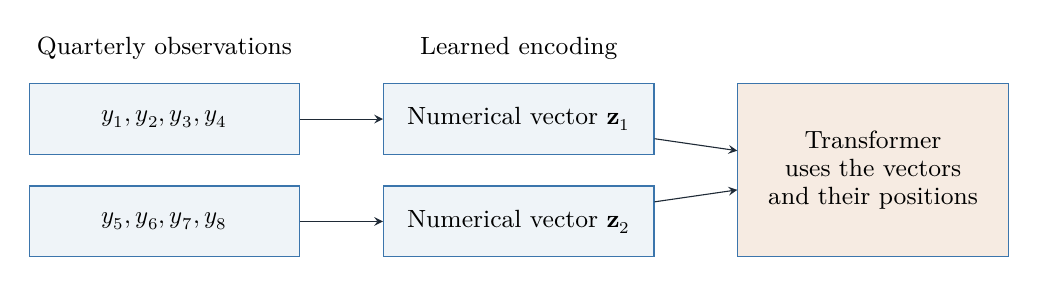
\begin{tikzpicture}[>=stealth,every node/.style={font=\fontsize{9}{10}\selectfont,align=center},
box/.style={draw=MonashBlue,fill=MonashBlue!8,text width=3.2cm,minimum height=.9cm}]
\node at (0,0.75) {Quarterly observations};
\node[box] (a) at (0,-.15) {$y_1,y_2,y_3,y_4$};
\node[box] (b) at (0,-1.45) {$y_5,y_6,y_7,y_8$};
\node[box] (e1) at (4.5,-.15) {Numerical vector $\mathbf{z}_1$};
\node[box] (e2) at (4.5,-1.45) {Numerical vector $\mathbf{z}_2$};
\node at (4.5,.75) {Learned encoding};
\node[box,fill=Orange!12,minimum height=2.2cm] (m) at (9,-.8) {Transformer\\uses the vectors\\and their positions};
\draw[->] (a)--(e1);
\draw[->] (b)--(e2);
\draw[->] (e1)--(m);
\draw[->] (e2)--(m);
\end{tikzpicture}
\end{document}
